%%%%%%%%%%%%%%%%%%%%%%%%%%%%%%%%%%%%%%%%%%%%%%%%%%%%%%%%%%%%%%%%%%%%%%%%%%%%%%%
%
%%%%%%%%%%%%%%%%%%%%%%%%%%%%%%%%%%%%%%%%%%%%%%%%%%%%%%%%%%%%%%%%%%%%%%%%%%%%%%%
\section{Gentle introduction to the data fitting.} \SecLabel{FittingGentleIntroducion}

The aim of this section is to briefly introduce the basic concept of
data fitting, its key terminology and difficulties which might arise in scattering data fit.
Users wanting to find out more about minimization (also called
maximization or optimization methods depending on the formulations and objectives) 
or looking for more rigorous discussion than provided in this manual
are referred to \cite{Antoniou2007, mntutorial}

\subsection{Toy scattering experiment.}

Fig.~\ref{fig:toyfit_data},left shows scattering intensity map in arbitrary units  
as a function of (x,y) of the detector ``measured'' in toy scattering experiment.

\begin{figure}[!p]
  \centering
    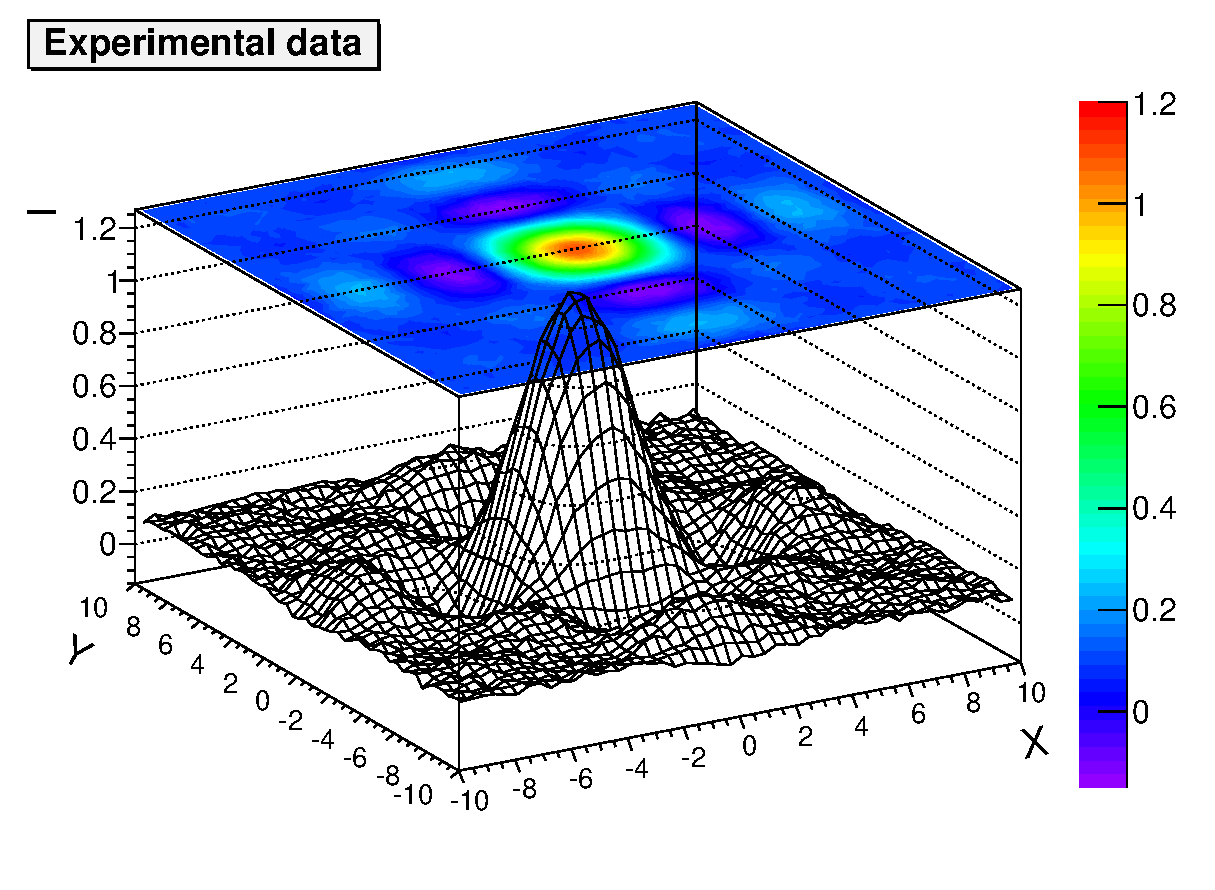
\includegraphics[width=0.49\textwidth]{Figures/toyfit_expdata.eps}
    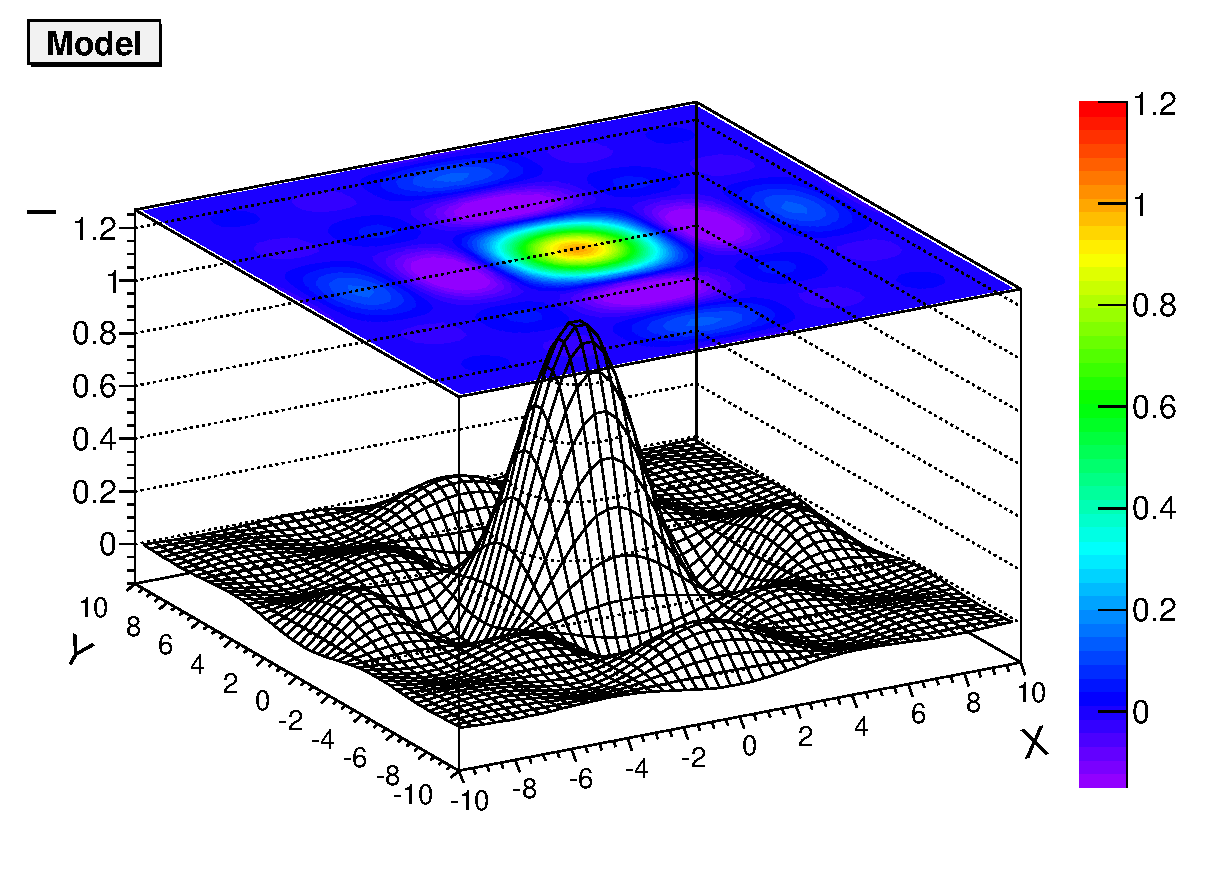
\includegraphics[width=0.49\textwidth]{Figures/toyfit_simdata.eps}
  \caption{Intensity as a function of (x,y) detector coordinates  obtained from 
  toy experiment (left) and from the toy simulation (right).   }
  \label{fig:toyfit_data}
  \vspace*{4mm}
    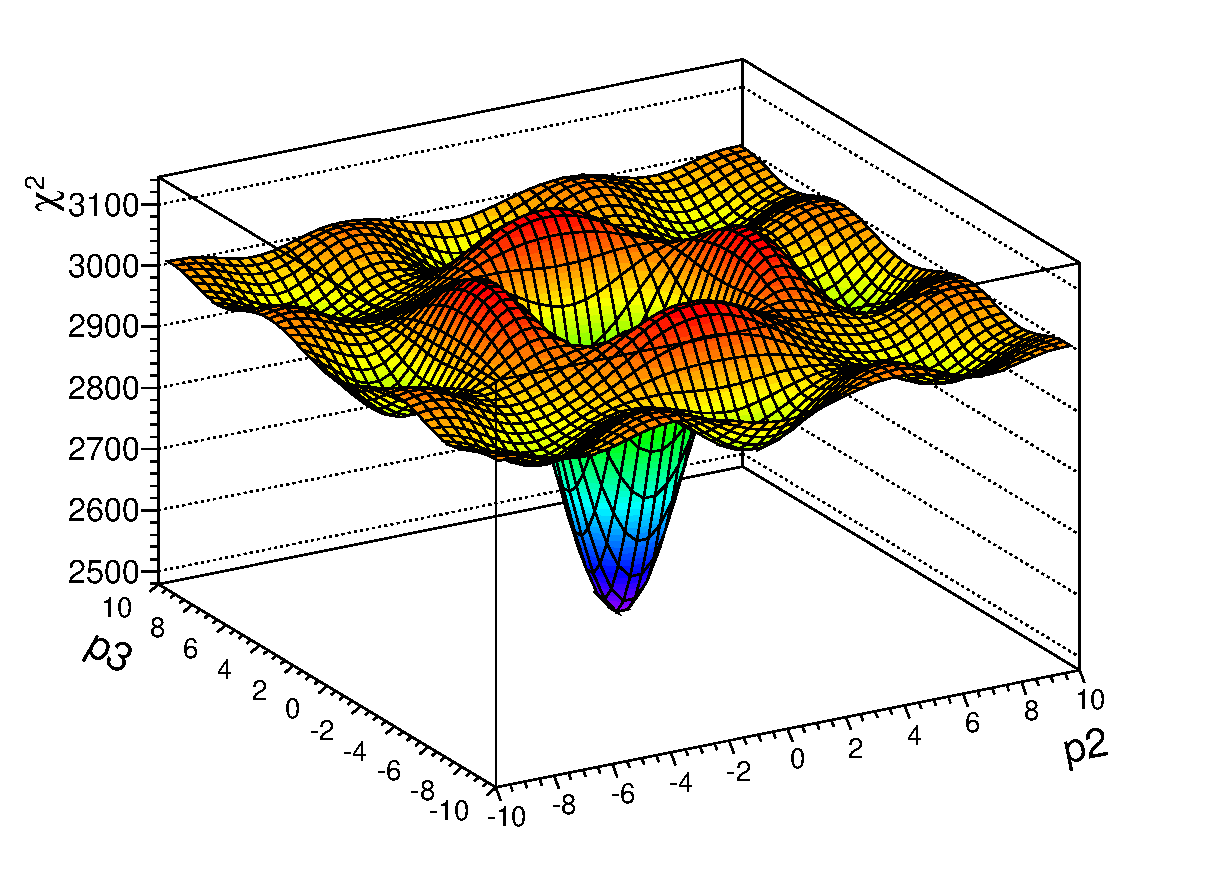
\includegraphics[width=0.49\textwidth]{Figures/toyfit_chi2_p23.eps}
    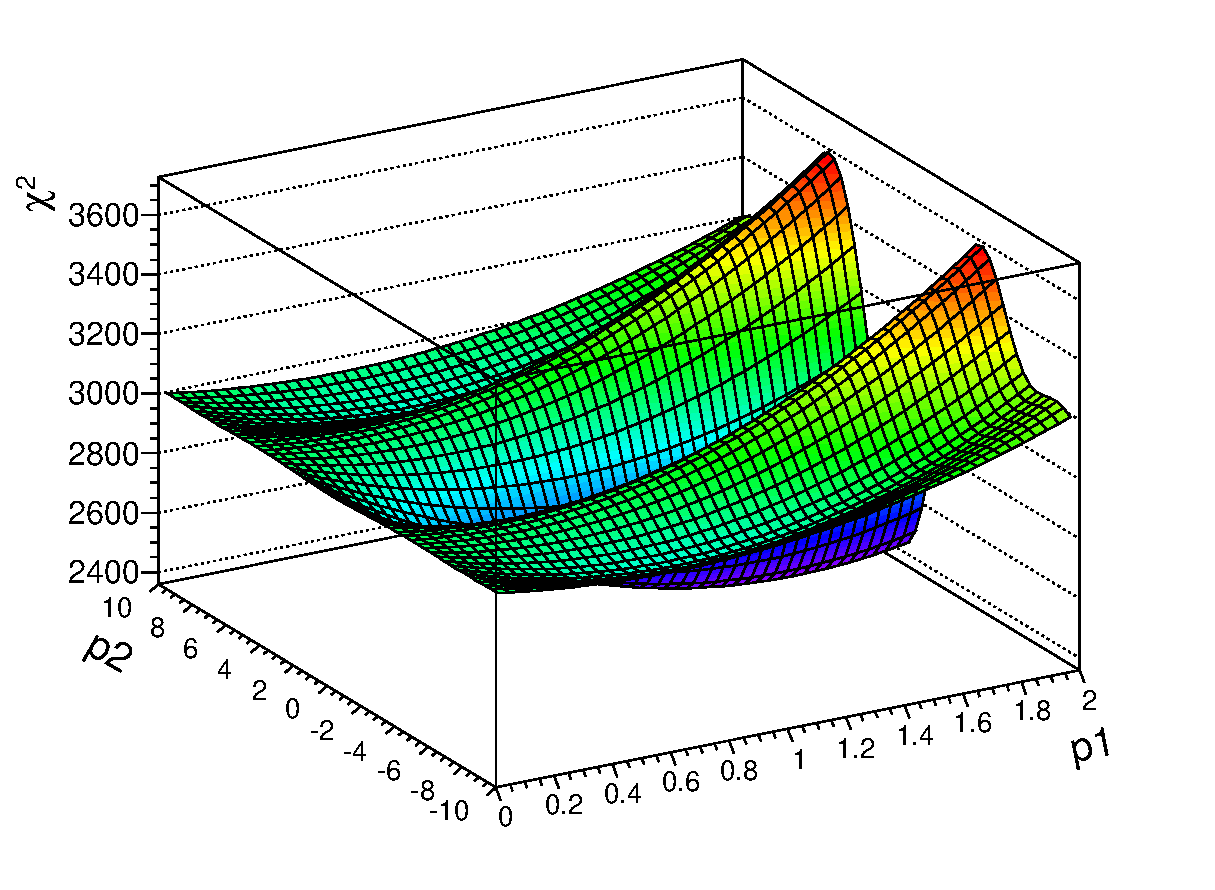
\includegraphics[width=0.49\textwidth]{Figures/toyfit_chi2_p12.eps}
  \caption{$\chi^{2}$ value calculated between experimental and simulated data
  as a function of $p_2,p_3$ parameters (left) or $p_1,p_2$ 
  parameters (right) used in the model.   }
  \label{fig:toyfit_chi2}
\end{figure}


Scattering picture presented reminds some of GISAS patterns, nevertheless it is
generated using simple function
$$I(x,y) = G(0.1,~0.01) + \frac{sin(x)}{x} \cdot \frac{sin(y)}{y}$$
Here $G(0.1, 0.01)$ is a random variable distributed according to the Gaussian distribution
with mean 0.1 and $\sigma=0.01$.
Constant $0.1$ symbolize our experimental background and constant $0.01$ is referred
to the detector noise. The rest of the formula represents our signal.

Lets define our model, namely specific mathematical function, to which we will fit our toy experimental data. By making an educated guess we assume that scattering intensity observed
in the experiment should be described with the help of $sinc$ function as follows
$$ I(x,y) = p_0 + p_1 \cdot  sinc(x - p_2) \cdot sinc(y - p_3) $$
The model has four parameters: $p_0$ describing background, $p_{1}$ describing signal strength
and $p_2,p_3$ responsible for the peak position.
Fig.~\ref{fig:toyfit_data},right shows the intensity as a function (x,y) calculated according
our model using fixed parameter set $p_0=0,p_1=1,p_2=0,p_3=0$. 

Two distributions look pretty much the same, however to find exact values of parameters which describe experimental data in the best way, one have to
\begin{itemize}
\item elaborate criteria for the difference between an actual data and its model
\item employ minimization procedure which will minimize that difference
\end{itemize}


\subsection{Objectives}

The goal is to obtain the best fit of an observed distribution
to a prediction by modifying a set of parameters from the
prediction. This problem can be one or multi-dimensional and also linear or
nonlinear. The quantity to minimize is often referred to as the
\textit{objective function}, whose expression depends on the
particular method, like the maximum likelihood, the $\chi^2$
minimization or the expected prediction error function. 

\begin{comment}
\subsubsection*{Maximum of likelihood.}
This is a popular method for parameters' estimations because the maximum likelihood estimators are approximately
unbiased and efficient for large data samples, under quite general
conditions.
We assume a sample  $\mathbf{x}=\{x_{1},x_{2},...,x_{n}\}$ of n independent and identically distributed
observations coming from probability density function $f(\mathbf{x}; \mathbf{p})$.
We assume $f(\mathbf{x}; \mathbf{p})$
to be known except for the parameters $\mathbf{p}=\{p_1,p_2,...,p_3\}$
The method of maximum likelihood takes the estimators to be
those values of $\mathbf{p}$ that maximize the likelihood function $\mathcal{L}$ as
$\mathcal{L}(\mathbf{\alpha})=\prod_{i=1}^N f(x_i;\mathbf{p})$.
Since it is easier to deal with a sum, we usually minimize
$-\text{ln}(\mathcal{L})$.
\end{comment}


\subsubsection*{$\chi^2$ or least squares minimization}
A simple dataset consist of $n$ data pairs 

\subsubsection*{Main features of minimization algorithm}



\subsection{Terminology.}

\noindent
{\bf Reference data} \\
Normally just experimental data or might be also simulated data
spoiled with the noise for purpose of testing of minimization algorithms.
\vspace*{1mm}

\noindent
{\bf Objective function} \\
Subject of minimization procedure.
\vspace*{1mm}

\noindent
{\bf Minimization} \\
Finding a best available values (i.e. local minimum) of some objective function. 
\vspace*{1mm}

\noindent
{\bf Number of degrees of freedom} \\
Number of data points - number of parameters in the fit.
\vspace*{1mm}

\noindent
{\bf Minimizer} \\
An algorithm which minimize objective function. 

